% =====================================================================
%  Bản tiếng Việt — CXR Nodule Detection
%
%  BẮT BUỘC biên dịch bằng XELATEX, không dùng pdflatex:
%      xelatex main_vi.tex && bibtex main_vi && xelatex main_vi.tex x2
%
%  pdflatex + inputenc KHÔNG đọc được ầ (U+1EA7), ị (U+1ECB) và nhiều chữ
%  khác. Nó không báo lỗi dừng mà LẶNG LẼ BỎ MẤT chữ — "Trần Thị" in ra
%  thành "Trn Th". Dùng nhầm trình biên dịch là hỏng mà không biết.
% =====================================================================
\documentclass[12pt,a4paper]{article}

\usepackage{fontspec}
\setmainfont{Times New Roman}
\usepackage{amsmath,amssymb}
\usepackage{booktabs}
\usepackage{graphicx}
\usepackage[margin=2.5cm]{geometry}
\usepackage{hyperref}
\hypersetup{colorlinks=true,linkcolor=blue,citecolor=blue,urlcolor=blue}
\usepackage{caption}
\captionsetup{labelfont=bf}
\renewcommand{\abstractname}{Tóm tắt}
\renewcommand{\refname}{Tài liệu tham khảo}
\renewcommand{\figurename}{Hình}
\renewcommand{\tablename}{Bảng}

\title{\textbf{Đánh giá phân tầng theo độ khó thấy trong phát hiện nốt phổi
trên X-quang ngực: mức cải thiện tổng thể tái lập được,\\
nhưng việc quy nó cho nhóm nào thì không}}

\author{Bùi Văn Xía \and Trần Thị Quỳnh Nga \\[4pt]
\normalsize Nghiên cứu viên độc lập, Việt Nam \\
\normalsize \texttt{buivanxia10@gmail.com}}
\date{}

\begin{document}
\maketitle

% =====================================================================
\begin{abstract}
\noindent
Phát hiện nốt phổi trên X-quang ngực thường được tóm lại bằng một chỉ số trung
bình duy nhất, chẳng hạn CPM. Vì nốt dễ thấy chiếm đa số, chỉ số đó chủ yếu
phản ánh năng lực trên những ca mà bác sĩ vốn đã nhìn ra. Chúng tôi đánh giá
phát hiện nốt trên bộ JSRT (247 ảnh, 154 nốt) theo từng mức trong thang độ khó
thấy năm bậc do bác sĩ gán, và gắn khoảng tin cậy bootstrap cho mọi con số.

Khử bóng xương --- biện pháp mà một công trình phân tầng trước đây đã đề xuất
nhưng chưa kiểm chứng --- làm tăng CPM tổng thể một cách tái lập được:
$+2{,}9$ điểm $[+0{,}7; +5{,}1]$ khi gộp năm hạt giống dưới kiểm chéo 10-fold,
và $+4{,}3$ $[+0{,}7; +8{,}6]$ dưới kiểm chéo bỏ-một. Nhưng \emph{mức cải thiện
đó nằm ở nhóm nào} thì không tái lập: 10-fold quy cho nhóm dễ thứ nhì, bỏ-một
quy cho nhóm khó thứ nhì. Chúng tôi báo cáo bất đồng này thay vì giải quyết nó,
bởi với 12--50 nốt mỗi nhóm, một ước lượng phân tầng không đủ vững để chống đỡ
một lập luận về cơ chế.

Ngay cả việc xác lập hiệu ứng tổng thể cũng đòi hỏi tách hai nguồn bất định
thường bị gộp làm một: bootstrap trên một lần chạy cho khoảng $[-0{,}9; +6{,}3]$
và che mất hiệu ứng, vì khoảng bốn điểm CPM dao động do khởi tạo ngẫu nhiên bị
hấp thụ vào cái mà khoảng đó trình bày như sai số lấy mẫu.

Độ nhạy ở nhóm khó thấy nhất nằm trong khoảng 0--8\% qua mọi cấu hình và cả hai
giao thức, và không nhúc nhích ngay cả dưới một tác động làm giảm một nửa năng
lực tổng thể. Khi đem nguyên mô hình sang 1.426 ảnh VinDr-CXR, CPM chỉ đạt
$16{,}5\%$ $[14{,}7; 18{,}3]$ so với $43{,}3\%$ nội bộ, ngay cả khi dung sai
đối sánh được nới rộng hơn mức dùng nội bộ.

Chúng tôi không nhận bất kỳ tính mới nào cho việc đánh giá phân tầng, cũng như
cho quan sát về mô hình nền đóng băng; cả hai đều đã được công bố trước.

\medskip
\noindent\textbf{Từ khoá:} X-quang ngực, phát hiện nốt phổi, phân tầng theo độ
khó thấy, phân tích FROC, khoảng tin cậy bootstrap, khả năng tái lập
\end{abstract}

% =====================================================================
\section{Giới thiệu}

Một nốt phổi hiện rõ trên phim X-quang không phải là ca cần người đọc thứ hai.
Ca đáng quan tâm là ca bác sĩ có thể bỏ sót: tổn thương nhỏ, tương phản thấp,
hoặc bị xương sườn và xương đòn che lấp. Các nghiên cứu hồi cứu về ung thư phổi
bị bỏ sót đều cho thấy tổn thương vốn nhìn thấy được khi xem lại --- Quekel và
cộng sự~\cite{quekel1999missrate} ghi nhận 19\% ca ung thư phổi bị bỏ sót trên
phim mà khi xem lại thì thấy được, với nguyên nhân chính là các cấu trúc xương
và mạch máu chồng lấp. Đó đúng là nhóm mà một hệ thống phát hiện cần nhắm tới,
và cũng đúng là nhóm mà khử bóng xương được kỳ vọng sẽ giúp.

Hiệu năng được báo cáo hiếm khi phản ánh điều này. Cách tóm tắt chuẩn là CPM,
tức độ nhạy trung bình tại một tập các mức dương tính giả cố định, tính gộp trên
toàn bộ số nốt. Khi nốt dễ chiếm đa số --- điều đúng với mọi bộ dữ liệu công
khai mà chúng tôi biết --- CPM chủ yếu đo năng lực trên những ca ít giá trị lâm
sàng. Một hệ thống hoàn toàn có thể đạt CPM đẹp trong khi gần như không phát
hiện được gì ở nhóm khó.

Bộ JSRT cho phép kiểm chứng trực tiếp điều này, vì mỗi nốt mang một mức độ khó
thấy từ 1 (cực khó thấy) đến 5 (rõ ràng), do ba bác sĩ chuyên khoa lồng ngực độc
lập gán. Thang này không chỉ là cảm nhận chuyên gia: trong chính nghiên cứu quan
sát viên của bộ dữ liệu, điểm tin cậy trung bình của 20 bác sĩ đọc cùng những ca
đó tương quan với mức độ khó thấy được gán ở $r = 0{,}999$~\cite{shiraishi2000jsrt}.
Trục phân tầng chúng tôi dùng vì thế neo vào độ khó phát hiện đo được ở người
thật, chứ không phải một cách chia nhóm tuỳ tiện.

Bài này dùng thang đó theo hai cách. Thứ nhất, báo cáo độ nhạy theo từng nhóm
thay vì gộp chung. Thứ hai, và quan trọng hơn, gắn khoảng tin cậy cho mọi con số
phân tầng.

Bước thứ hai hoá ra quan trọng hơn bước thứ nhất. Chia 154 nốt thành năm mức để
lại 25 nốt ở nhóm khó nhất và 12 nốt ở nhóm dễ nhất. Ở những cỡ mẫu đó, chỉ một
nốt đổi trạng thái đã làm độ nhạy báo cáo dịch chuyển bốn đến tám điểm phần trăm.
Chênh lệch cỡ đó vẫn thường xuyên được công bố như một cải tiến. Chúng tôi cho
thấy không nên làm vậy.

\paragraph{Đóng góp.}
\begin{enumerate}
  \item So sánh các cấu hình phát hiện trên JSRT theo từng mức độ khó thấy,
        trong đó mọi con số --- cả tổng thể lẫn phân tầng --- đều kèm khoảng
        tin cậy bootstrap.
  \item Một quy trình tách bất định do huấn luyện khỏi bất định do lấy mẫu:
        trung bình qua các hạt giống trước, rồi mới bootstrap theo ảnh quanh
        trung bình đó. Chúng tôi cho thấy báo cáo riêng lẻ từng loại đều gây
        hiểu sai, theo cả hai chiều.
  \item Đo dao động giữa các lần chạy do khởi tạo ngẫu nhiên, và thấy nó tương
        đương về độ lớn với chính các hiệu ứng kiến trúc đang được nghiên cứu.
  \item Bằng chứng rằng nhóm khó thấy nhất kháng lại mọi cấu hình được thử, và
        không nhúc nhích ngay cả dưới tác động làm giảm một nửa năng lực tổng thể.
  \item Kiểm chứng trực tiếp lời giải thích thông thường về việc vì sao tăng
        cường dữ liệu làm hỏng bộ phát hiện dùng backbone đóng băng, bằng cách
        mở băng một phần backbone.
  \item Kiểm định ngoại trên VinDr-CXR, trong đó khác biệt về dung sai đối sánh
        được đo và loại bỏ, để mức sụt giảm được quy cho khả năng tổng quát hoá
        chứ không cho việc đổi tiêu chí.
\end{enumerate}

Chúng tôi không nhận tính tiên phong. Horry và cộng sự~\cite{horry2023fullres}
đã phân tích JSRT theo độ khó thấy bằng kiến trúc mã hoá--giải mã toàn phân giải,
quan sát đúng sự sụp đổ ở các mức thấp nhất mà chúng tôi cũng thấy, và đề xuất
chính biện pháp mà chúng tôi đánh giá: \emph{``Các kỹ thuật khử xương sườn và
xương\ldots có thể được kỳ vọng cải thiện cả độ nhạy của thuật toán này lẫn giảm
tỷ lệ dương tính giả.''} Họ không đánh giá nó, mà cho biết công việc đang được
tiến hành. Bài này kiểm chứng đề xuất đó. Mức cải thiện là có thật và tái lập
được qua hai giao thức kiểm chéo; nhóm nào đóng góp mức cải thiện đó thì không
tái lập, và nhóm mà chính phân tích của họ chỉ ra là vấn đề thì không dịch
chuyển dưới cả hai giao thức.

% =====================================================================
\section{Công trình liên quan}

\paragraph{Phát hiện nốt trên X-quang ngực.}
Lĩnh vực này hiện do các bộ phát hiện và mạng phân đoạn học sâu chi phối, với
NODE21~\cite{sogancioglu2024node21} là chuẩn đối sánh dễ thấy nhất. Hiệu năng
được báo cáo hầu như luôn là một con số tổng thể duy nhất, tính gộp trên toàn bộ
số nốt. Ở những chỗ có phân tích theo độ khó, như trong Horry và cộng
sự~\cite{horry2023fullres}, con số tổng thể lộ ra là đang che giấu thất bại gần
như hoàn toàn ở các ca khó nhất.

\paragraph{Đánh giá phân tầng theo độ khó thấy.}
Việc phân tầng kết quả JSRT theo thang độ khó thấy không mới. Horry và cộng
sự~\cite{horry2023fullres} đánh giá kiến trúc mã hoá--giải mã toàn phân giải theo
từng mức và quan sát đúng sự sụp đổ ở các mức thấp mà chúng tôi cũng thấy. Công
trình đó đề xuất khử bóng xương như một hướng khắc phục khả dĩ nhưng không đánh
giá nó. Nghiên cứu của chúng tôi nên được đọc như một phép kiểm chứng đề xuất
đó, chứ không phải một ý tưởng độc lập.

Công trình ấy cũng minh hoạ --- một cách minh bạch và bằng chính lời họ --- vì
sao việc phân tầng ảnh hưởng tới cách đọc kết quả. Con số tổng quát hoá ngoại
mạnh nhất của họ, 76,7\% độ nhạy tại 7,6 dương tính giả mỗi ảnh, đạt được
\emph{``khi các nốt rất khó thấy và cực khó thấy bị loại khỏi dữ liệu huấn luyện
JSRT''}~\cite{horry2023fullres}, và họ ghi rõ cấu hình tốt nhất của mình đã loại
các nhóm đó. Chúng tôi nêu điều này không phải để phê phán, vì nó được trình bày
thẳng thắn trong nguồn, mà vì nó làm luận điểm trở nên cụ thể: một con số hiệu
năng luôn có điều kiện là những nhóm độ khó nào nằm trong phạm vi tính toán, và
hai nhóm khó nhất thường là hai nhóm nằm ngoài.

\paragraph{Khử bóng xương.}
Khử bóng xương sườn và xương đòn là bước tiền xử lý đã được xác lập. Các cách
tiếp cận học máy sớm huấn luyện autoencoder và mạng tích chập để hồi quy ảnh mô
mềm~\cite{gusarev2017bonesup}, còn các mô hình sinh gần đây tái tạo ảnh không
xương với độ trung thực cao --- Ibrahim và cộng sự~\cite{ibrahim2025bonesup} báo
cáo SSIM $0{,}99$ trên JSRT. Toàn bộ nhánh nghiên cứu này được đánh giá theo chất
lượng tái tạo ảnh, chứ không theo việc khử xương có cải thiện \emph{phát hiện}
tổn thương hay không, và chưa bao giờ theo từng mức độ khó thấy. Khoảng trống mà
chúng tôi lấp chính là ở phía hạ nguồn đó.

\paragraph{Mô hình nền cho ảnh y khoa.}
RAD-DINO~\cite{perezgarcia2024raddino} là một vision transformer tự giám sát
huấn luyện trên kho ảnh X-quang ngực lớn. Có một chi tiết quan trọng cho việc
diễn giải kết quả của chúng tôi. RAD-DINO như được đề xuất huấn luyện trên 838
nghìn ảnh, trong đó 90 nghìn thuộc một nhóm dữ liệu riêng tư; nhóm tác giả huấn
luyện thêm một bản chỉ dùng dữ liệu công khai để phát hành. Checkpoint
\texttt{microsoft/rad-dino} mà chúng tôi dùng chính là bản công khai đó, với các
tập thành phần cộng lại vào khoảng 748 nghìn ảnh. Vì vậy chúng tôi không gán con
số 838 nghìn cho mô hình thực sự được chạy.

Muthyala và cộng sự~\cite{muthyala2026frozen} khảo sát năm vision transformer
đóng băng, trong đó có RAD-DINO, và cho thấy tín hiệu tổn thương nhỏ bị loại bỏ
ở bước gộp toàn cục nhưng vẫn khôi phục được từ các token vùng. Bằng chứng của họ
là AUC phân loại trên NIH-CXR14, MIMIC-CXR, Emory-CXR và ChestX-Det10; của chúng
tôi là phát hiện tổn thương trên JSRT phân tầng theo độ khó thấy. Hai hướng bổ
trợ cho nhau, và chúng tôi coi kết quả của họ là phát hiện có trước chứ không
phải của mình. Cần lưu ý rằng bộ giải mã của chúng tôi đọc token vùng chứ không
đọc token lớp --- đúng cấu hình mà phân tích của họ xác định là \emph{giữ được}
tín hiệu --- nên thất bại dai dẳng ở nhóm khó nhất trong nghiên cứu này không
giải thích được chỉ bằng cơ chế gộp toàn cục.

\paragraph{Chuẩn đối sánh và nhiễm chéo dữ liệu.}
JSRT nằm trong dữ liệu huấn luyện của NODE21~\cite{sogancioglu2024node21}, chuẩn
đối sánh hiện hành cho phát hiện nốt trên X-quang ngực. Do đó kết quả trên JSRT
không thể so sánh trực tiếp với các mô hình đã thấy dữ liệu huấn luyện NODE21,
và chúng tôi không thực hiện phép so sánh nào như vậy.

% =====================================================================
\section{Dữ liệu và phương pháp}

\subsection{Dữ liệu}

\paragraph{JSRT.}
Bộ JSRT~\cite{shiraishi2000jsrt} gồm 247 phim X-quang ngực thẳng sau--trước thu
thập từ 14 cơ sở y tế: 154 phim có một nốt phổi đơn độc đã xác nhận bằng CT, và
93 phim không có nốt. Phim được số hoá ở $2048 \times 2048$ với điểm ảnh
0,175\,mm. Mỗi nốt mang mức độ khó thấy từ 1 đến 5 do ba bác sĩ chuyên khoa lồng
ngực gán, phản ánh kích thước, mật độ và mức độ bị các cấu trúc phía trên che
lấp. Phân bố không đều --- lần lượt 25, 29, 50, 38 và 12 nốt ở các mức 1 đến 5
--- và hai nhóm biên nhỏ tới mức mọi chênh lệch ở đó phải được diễn giải hết sức
thận trọng. Mỗi ca dương tính chỉ chứa đúng một nốt; đường kính dao động từ 5
đến 60\,mm với trung vị 15\,mm.

\paragraph{NIH ChestX-ray14.}
112.120 ảnh từ ChestX-ray14~\cite{wang2017chestxray} được dùng để tiền huấn
luyện backbone ResNet-34. Nhãn của bộ này được khai thác tự động từ báo cáo và
đã được ghi nhận là có nhiễu~\cite{oakdenrayner2020exploring}; chúng tôi chỉ dùng
nó để học biểu diễn, không bao giờ để đánh giá.

\paragraph{Ảnh khử bóng xương.}
241 cặp phim có và không có bóng xương được dùng để huấn luyện mạng khử xương mô
tả bên dưới. Ảnh gốc là phim JSRT~\cite{shiraishi2000jsrt}; ảnh đã khử xương là
bộ BSE-JSRT do Juhász và cộng sự~\cite{juhasz2010bse} tạo ra. JSRT có 247 ảnh còn
bản khử xương phủ 241 trong số đó. Chúng tôi lấy bộ cặp này qua một kênh phân
phối lại trên Kaggle, đó là điểm truy cập chứ không phải nguồn.

\subsection{Khung phát hiện}

Chúng tôi xử lý bài toán phát hiện như hồi quy bản đồ nhiệt. Tâm mỗi nốt sinh ra
một đích Gauss ($\sigma = 8$ điểm ảnh) trên lưới đầu ra bước 4; giá trị tại điểm
ảnh tâm sau khi làm tròn được ép bằng đúng 1,0, nếu không lớp dương không bao giờ
được biểu diễn chính xác và mạng không học được gì. Dự đoán được giải mã bằng
triệt tiêu phi cực đại với khoảng cách đỉnh tối thiểu 10 điểm ảnh.

Huấn luyện cực tiểu hoá hàm mất mát focal bình phương trung bình. Gradient được
cắt theo chuẩn 5,0. \textbf{Độ chính xác hỗn hợp bị tắt}: khi bật tự động độ
chính xác hỗn hợp, hàm mất mát tràn xuống đúng bằng không và mạng hoàn toàn không
học. Chúng tôi ghi lại điều này vì nó tiêu tốn rất nhiều thời gian gỡ lỗi và, theo
hiểu biết của chúng tôi, chưa được ghi nhận cho lớp hàm mất mát này.

\subsection{Các cấu hình được so sánh}

\begin{description}
  \item[Nền tảng.] Bộ mã hoá ResNet-34 tiền huấn luyện trên NIH ChestX-ray14,
        đầu vào một kênh xám.
  \item[Khử xương kèm chú ý.] Cùng bộ mã hoá, thêm kênh đầu vào thứ hai mang ảnh
        đã khử xương do một U-Net huấn luyện trên dữ liệu cặp sinh ra, cùng các
        khối chú ý CBAM~\cite{woo2018cbam}.
  \item[Mô hình nền.] Checkpoint công khai \texttt{microsoft/rad-dino} (87 triệu
        tham số theo công bố; 86,6 triệu trong trọng số phát hành) với toàn bộ
        trọng số đóng băng, dùng như bộ trích xuất đặc trưng. Ba kênh đầu vào là
        [ảnh gốc, ảnh khử xương, ảnh gốc]. Một bộ giải mã tích chập nhẹ được
        huấn luyện trên đặc trưng trích xuất.
\end{description}

\subsection{Giao thức đánh giá}

Chúng tôi báo cáo phân tích FROC. Một phát hiện được tính là trúng khi đỉnh của
nó nằm trong bán kính 15\,mm quanh tâm nốt thật; mỗi nốt chỉ được ghép nhiều nhất
một lần, và các đỉnh không ghép được là dương tính giả. CPM là độ nhạy trung bình
tại các mức 0,125; 0,25; 0,5; 1,0; 2,0 và 4,0 dương tính giả mỗi ảnh.

Độ nhạy phân tầng dùng \emph{cùng các ngưỡng vận hành} với đường cong FROC tổng
thể. Điểm này rất dễ làm sai: tính độ nhạy phân tầng bằng cách đếm mọi phát hiện
mà không áp ngưỡng FROC sẽ thổi phồng các con số đáng kể và phá vỡ tính đơn điệu
của chúng theo độ khó thấy. Chúng tôi đã mắc lỗi này hai lần trong quá trình phát
triển trước khi phát hiện ra.

Giao thức chính là kiểm chéo 10-fold với hạt giống cố định; kiểm chéo bỏ-một được
dùng để đối chứng. Các fold được chia \emph{theo ảnh}, sao cho mọi biến thể tăng
cường của một ảnh luôn nằm cùng phía; chia theo biến thể sẽ làm rò rỉ dữ liệu
huấn luyện sang fold kiểm tra.

\subsection{Định lượng bất định}
\label{sec:bootstrap-vi}

Mọi con số chúng tôi báo cáo đều kèm khoảng tin cậy bootstrap 95\% hiệu chỉnh độ
lệch và gia tốc (BCa) trên $B = 2000$ lần lấy mẫu với hạt giống cố định. Ba lựa
chọn thiết kế sau là thiết yếu; làm sai bất kỳ điểm nào sẽ cho khoảng hẹp hơn
thực tế.

\paragraph{Lấy mẫu lại theo ảnh, không theo nốt.}
Ngưỡng vận hành FROC được định nghĩa bởi số dương tính giả \emph{trên mỗi ảnh}.
Lấy mẫu lại từng nốt riêng lẻ làm số ảnh không còn xác định và tách các dương tính
giả khỏi ảnh sinh ra chúng, khiến ngưỡng mất ý nghĩa. Vì vậy chúng tôi lấy mẫu
lại các ảnh có hoàn lại; một ảnh được chọn sẽ đóng góp toàn bộ số nốt và toàn bộ
dương tính giả của nó.

\paragraph{Tính lại ngưỡng trong từng lần lấy mẫu.}
Giữ nguyên ngưỡng của mẫu gốc là bỏ qua chính độ bất định của việc ước lượng
ngưỡng đó. Chúng tôi đo chi phí của lựa chọn này bằng cách chạy cả hai biến thể
trên những mẫu lấy lại giống hệt nhau, chỉ khác ở việc ngưỡng có được tính lại
hay không: giữ ngưỡng cố định làm khoảng tin cậy hẹp đi 2,9\% tính trung bình và
tới 11,8\% tại một số điểm vận hành. Hiệu ứng có thật nhưng khiêm tốn, và chúng
tôi báo cáo độ lớn đo được thay vì khẳng định rằng nó lớn.

\paragraph{So sánh phải bắt cặp.}
Khi so sánh hai cấu hình, chúng tôi lấy lại cùng một tập chỉ số ảnh cho cả hai và
lập khoảng tin cậy trên \emph{hiệu số}. Cả hai cấu hình được đánh giá trên cùng
247 ảnh, nên phần lớn phương sai là chung và triệt tiêu lẫn nhau.

Vì các so sánh phân tầng liên quan năm nhóm tại nhiều điểm vận hành, chúng tôi
không hiệu chỉnh đa so sánh và coi các kết quả đó là mang tính thăm dò.

Hai hạn chế của chính quy trình cần được nêu rõ. Hệ số gia tốc BCa được ước lượng
bằng jackknife qua các ảnh, vốn giả định thống kê biến thiên trơn khi xoá bỏ từng
quan sát; việc tính lại ngưỡng khiến nó chỉ trơn từng khúc, nên các đầu mút khoảng
mang sai số xấp xỉ ngoài nhiễu Monte Carlo. Ngoài ra, ước lượng gộp hạt giống ở
mục~\ref{sec:hai-nhieu-vi} lan truyền bất định do lấy mẫu ảnh nhưng không lan
truyền bất định của việc ước lượng trung bình đó từ chỉ năm hạt giống.

% =====================================================================
\section{Kết quả}

\subsection{Hiệu năng tổng thể}

\begin{table}[t]
\centering
\caption{Kiểm chéo bỏ-một trên JSRT. Hai dòng RAD-DINO là các lần chạy có gieo
hạt và có lưu điểm thô theo ảnh, nên khoảng tin cậy tính được; hai dòng ResNet-34
là các lần chạy đơn lẻ trước đây không gieo hạt và không lưu điểm, tự thân chúng
không xác lập điều gì.}
\label{tab:loocv-vi}
\begin{tabular}{llc}
\toprule
Cấu hình & Kiến trúc & CPM (\%) [KTC 95\%] \\
\midrule
\multicolumn{3}{l}{\emph{Có gieo hạt, tính được khoảng tin cậy:}} \\
3 kênh lặp        & RAD-DINO (đóng băng)          & 40,3 $[34{,}0; 48{,}0]$ \\
+ khử bóng xương  & RAD-DINO (đóng băng) + U-Net  & 44,6 $[37{,}7; 51{,}3]$ \\
\midrule
\multicolumn{3}{l}{\emph{Chạy đơn lẻ trước đây, không có khoảng tin cậy:}} \\
Nền tảng                  & ResNet-34                & 29,5 \\
+ khử xương + chú ý       & ResNet-34 + U-Net + CBAM & 34,2 \\
\bottomrule
\end{tabular}
\end{table}

Dưới kiểm chéo bỏ-một, khử bóng xương cho $+4{,}3$ điểm CPM $[+0{,}7; +8{,}6]$,
một khoảng không chứa số không và nhất quán về dấu lẫn độ lớn với $+2{,}9$
$[+0{,}7; +5{,}1]$ thu được từ năm hạt giống dưới 10-fold. Hiệu ứng tổng thể tái
lập qua hai giao thức.

\begin{figure}[t]
\centering
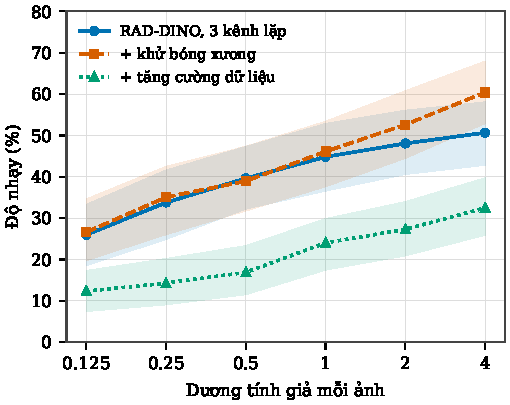
\includegraphics{fig/fig_froc_vi.pdf}
\caption{Đường cong FROC của ba cấu hình RAD-DINO (10-fold). Dải tô là khoảng
tin cậy bootstrap 95\% theo ảnh. Đường có khử xương và đường 3 kênh chồng lấn
trên phần lớn dải; cấu hình có tăng cường tách hẳn khỏi cả hai. Kiểu nét và dấu
mã hoá cấu hình bên cạnh màu, nên hình vẫn đọc được khi in đen trắng.}
\label{fig:froc-vi}
\end{figure}

\subsection{Dao động giữa các lần chạy}
\label{sec:nhieu-vi}

Chạy lại một cấu hình với cùng hạt giống và cùng tệp cấu hình cho CPM 40,5\%
trong khi con số ghi nhận trước đó là 36,5\%. Nguyên nhân là hạt giống chi phối
cách chia fold nhưng chưa bao giờ được áp cho việc khởi tạo trọng số của đầu phát
hiện. Qua năm hạt giống, cấu hình 3 kênh đạt $40{,}4 \pm 1{,}0$ và cấu hình có
khử xương đạt $43{,}3 \pm 1{,}4$ điểm CPM.

Điều này quyết định cách đọc mọi kết quả còn lại. Bốn điểm dao động chỉ do khởi
tạo đã tương đương với chính những mức cải thiện thường được công bố trên chuẩn
đối sánh này, nên một lần huấn luyện đơn lẻ không thể xác lập được điều gì.

\subsection{Tách bất định huấn luyện khỏi bất định lấy mẫu}
\label{sec:hai-nhieu-vi}

Hai loại bất định khác nhau tác động lên các con số này, và gộp chúng lại dẫn tới
sai lầm theo cả hai chiều.

Bất định do huấn luyện trả lời câu hỏi liệu chạy lại có cho cùng kết quả hay
không, và được đo bằng cách lặp thí nghiệm qua nhiều hạt giống. Bất định do lấy
mẫu trả lời liệu kết quả có giữ được trên một tập 247 ảnh khác hay không, và được
đo bằng bootstrap theo ảnh. Báo cáo riêng lẻ từng loại đều gây hiểu sai. Khoảng
bootstrap từ một lần huấn luyện hấp thụ nhiễu khởi tạo vào cái mà nó trình bày
như bất định lấy mẫu, nên rộng quá mức. Độ lệch chuẩn qua các hạt giống lại được
tính trên một tập ảnh cố định duy nhất nên không nói gì về khả năng tổng quát hoá.

Vì vậy chúng tôi lấy \emph{hiệu số trung bình qua các hạt giống} làm ước lượng
chính và bootstrap ảnh quanh nó: trong mỗi lần lấy mẫu, cùng một tập chỉ số ảnh
được áp cho cả mười lần chạy, hiệu số từng hạt giống được tính rồi lấy trung
bình. Cách này khử nhiễu huấn luyện bằng trung bình trong khi vẫn giữ nguyên bất
định do lấy mẫu.

Áp dụng cho khử bóng xương: hiệu số là $+2{,}9$ điểm CPM với khoảng tin cậy 95\%
là $[+0{,}7; +5{,}1]$, và dương ở cả năm hạt giống. Đáng chú ý, bootstrap trên
một hạt giống của chính dữ liệu đó cho $+2{,}8$ với khoảng $[-0{,}9; +6{,}3]$
--- chứa số không. Hiệu ứng không hề vắng mặt trong phân tích đó; nó bị nhiễu
huấn luyện che khuất, và ước lượng gộp đã loại bỏ được lớp nhiễu ấy.

\begin{figure}[t]
\centering
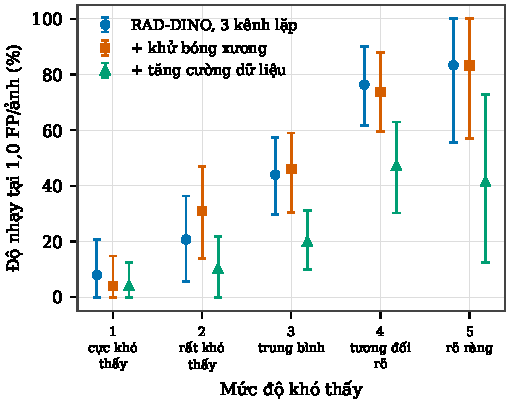
\includegraphics{fig/fig_strat_vi.pdf}
\caption{Độ nhạy tại 1,0 dương tính giả mỗi ảnh theo từng mức độ khó thấy, kèm
khoảng tin cậy bootstrap 95\% theo ảnh. Các khoảng đều rộng ở mọi mức và chồng
lấn gần như khắp nơi --- và đó chính là điều đáng nói: với 12--50 nốt mỗi nhóm,
chênh lệch ở cỡ thường được công bố như cải tiến là không phân giải được.}
\label{fig:strat-vi}
\end{figure}

\subsection{Nhóm nào hưởng lợi thì không ổn định qua các giao thức}
\label{sec:batondinh-vi}

Hiệu ứng tổng thể tái lập. Việc quy nó cho nhóm nào thì không.

\begin{table}[t]
\centering
\caption{Mức tăng do khử bóng xương theo từng mức độ khó thấy tại 1,0 dương tính
giả mỗi ảnh, dưới hai giao thức. In đậm là khoảng không chứa số không. Hai giao
thức đồng ý về con số tổng thể nhưng bất đồng về nhóm nào tạo ra nó.}
\label{tab:batondinh-vi}
\begin{tabular}{lcc}
\toprule
Mức độ khó thấy & 10-fold, gộp 5 hạt giống & Bỏ-một, 1 hạt giống \\
\midrule
1 --- cực khó thấy   & $-0{,}8$ & $+0{,}0$ \\
2 --- rất khó thấy   & $+1{,}4$ & $\mathbf{+17{,}2}$ $[+3{,}8; +31{,}0]$ \\
3 --- trung bình     & $+1{,}6$ & $+4{,}0$ \\
4 --- tương đối rõ   & $\mathbf{+6{,}3}$ $[+1{,}9; +11{,}4]$ & $+13{,}2$ $[0{,}0; +24{,}5]$ \\
5 --- rõ ràng        & $+10{,}0$ & $-16{,}7$ \\
\midrule
CPM tổng thể & $\mathbf{+2{,}9}$ $[+0{,}7; +5{,}1]$ & $\mathbf{+4{,}3}$ $[+0{,}7; +8{,}6]$ \\
\bottomrule
\end{tabular}
\end{table}

\begin{figure}[t]
\centering
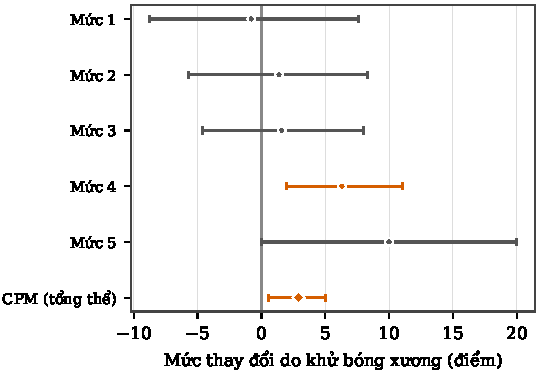
\includegraphics{fig/fig_forest_vi.pdf}
\caption{Hiệu ứng của khử bóng xương theo từng mức độ khó thấy dưới kiểm chéo
10-fold, trung bình qua năm hạt giống, kèm khoảng tin cậy bootstrap 95\% theo
ảnh; khoảng không chứa số không được vẽ màu. Mức tăng tổng thể là thật và tái
lập được dưới bỏ-một, nhưng mẫu hình phân tầng này thì không:
dưới bỏ-một mức tăng chuyển sang mức 2 và mức 5 trở thành âm
(Bảng~\ref{tab:batondinh-vi}). Hãy đọc dòng tổng thể như phát hiện, còn các
dòng phân tầng như kết quả tạm thời.}
\label{fig:forest-vi}
\end{figure}

Dưới 10-fold gộp hạt giống, nhóm duy nhất vượt số không là mức 4 và mức 5 tăng 10
điểm; dưới bỏ-một với một hạt giống, mức 2 vượt số không với mức tăng 17 điểm
trong khi mức 5 \emph{mất} 17 điểm. Cả hai phân tích dùng cùng ảnh, cùng mô hình
và cùng kênh khử xương.

Chúng tôi coi ước lượng 10-fold gộp hạt giống là đáng tin hơn, vì nó trung bình
qua năm hạt giống trong khi mục~\ref{sec:nhieu-vi} đã đo được khoảng bốn điểm CPM
dao động mà một lần chạy đơn lẻ không thể khử. Nhưng chúng tôi không cho rằng nên
gạt bất đồng này sang một bên. Đó chính là luận điểm của bài quay lại áp dụng cho
chính kết quả của bài: với 12 đến 50 nốt mỗi nhóm, một ước lượng phân tầng không
đủ ổn định để chống đỡ một khẳng định về \emph{nơi} một phương pháp phát huy tác
dụng, ngay cả khi hiệu ứng tổng thể mà nó tạo ra là vững chắc. Người đọc --- và
cả chúng tôi --- nên cưỡng lại cám dỗ dựng một câu chuyện cơ chế trên một mẫu
hình phân tầng ở cỡ mẫu này.

Thứ sống sót qua cả hai giao thức thì hẹp hơn, và theo chúng tôi là đáng tin hơn:
khử bóng xương cải thiện CPM tổng thể vài điểm, và mức 1 không dịch chuyển trong
cả hai phân tích.

\subsection{Một tương phản đứng vững: tăng cường dữ liệu khi backbone đóng băng}
\label{sec:tangcuong-vi}

Không phải mọi chênh lệch đều tan trong nhiễu. Tăng cường dữ liệu trong khi
backbone vẫn đóng băng làm CPM giảm 22,1 điểm, với khoảng tin cậy 95\% là
$[-28{,}2; -16{,}1]$, và mọi điểm vận hành riêng lẻ đều loại trừ số không. Hiệu
ứng này lớn hơn một bậc so với nhiễu khởi tạo đo được ở mục~\ref{sec:nhieu-vi},
và chúng tôi báo cáo nó không chút dè dặt.

Các dòng phân tầng mang một quan sát mà chúng tôi không dự đoán trước. Mức suy
giảm đơn điệu theo độ khó thấy --- những nốt rõ nhất mất nhiều nhất, 41,7 điểm
--- còn mức 1 hoàn toàn không dịch chuyển: $+0{,}0$ với khoảng
$[-11{,}5; +11{,}5]$. Một tác động đủ mạnh để làm giảm một nửa năng lực tổng thể
vẫn để nhóm khó nhất đứng nguyên tại chỗ, bởi ở mức 4\% --- tức một nốt trên 25
--- gần như không còn gì để mất.

\subsection{Mở băng backbone loại bỏ phần lớn hình phạt}
\label{sec:tinhchinh-vi}

Mục~\ref{sec:tangcuong-vi} xác lập rằng tăng cường dữ liệu tốn 22 điểm CPM khi
backbone đóng băng, và đưa ra một lời giải thích: backbone đóng băng không thích
nghi được với ảnh đã biến đổi, nên ảnh tăng cường lệch khỏi phân bố mà đặc trưng
của nó được học. Lời giải thích đó dự đoán một điều kiểm chứng được. Nếu nó đúng,
cho phép backbone thích nghi sẽ loại bỏ hình phạt.

Chúng tôi mở băng bốn khối transformer cuối của RAD-DINO (28,4 trên 86,6 triệu
tham số của checkpoint) và lặp lại phép tương phản. Hai nhánh dùng thiết lập giống
hệt nhau --- bốn khối mở băng, 20 epoch, năm fold, lô 2, hạt giống 42 --- và chỉ
khác nhau ở việc có áp dụng tăng cường hay không.

\begin{table}[t]
\centering
\caption{Hình phạt của tăng cường dữ liệu dưới backbone đóng băng so với backbone
tinh chỉnh một phần. Trong mỗi dòng, hai nhánh dùng chung giao thức và chỉ khác ở
tăng cường; hai dòng dùng giao thức khác nhau nên chỉ so sánh được về mặt định
tính.}
\label{tab:tinhchinh-vi}
\begin{tabular}{lccc}
\toprule
Backbone & Không tăng cường & Có tăng cường & Hiệu số [KTC 95\%] \\
\midrule
Đóng băng (10-fold, 60 ep.)       & 43,3 & 21,2 & $-22{,}1$ $[-28{,}2; -16{,}1]$ \\
Mở 4 khối (5-fold, 20 ep.)        & 42,2 & 39,1 & $\phantom{0}-3{,}1$ $[-8{,}5; +2{,}1]$ \\
\bottomrule
\end{tabular}
\end{table}

Hình phạt giảm từ 22,1 điểm xuống 3,1, và khoảng tin cậy của phép tương phản sau
khi tinh chỉnh có chứa số không. Hai khoảng không chồng lấn nhau. Dự đoán được
xác nhận: phần lớn thiệt hại mà tăng cường gây ra cho hệ thống này là do backbone
không thể thích nghi, chứ không phải do bản thân việc tăng cường.

Hai điều giới hạn kết luận này. Các lần chạy tinh chỉnh dùng năm fold và 20 epoch
so với mười fold và 60 epoch của các lần chạy đóng băng, nên so sánh \emph{hai
hiệu số} là so sánh chéo giao thức chứ không phải một thí nghiệm có kiểm soát duy
nhất; trong từng dòng thì phép so sánh có kiểm soát. Ngoài ra, các nhánh tinh
chỉnh là chạy đơn lẻ, trong khi mục~\ref{sec:nhieu-vi} đo được khoảng bốn điểm
dao động --- đủ lớn để ảnh hưởng tới một hiệu số 3,1 điểm. Sự sụp đổ định tính từ
22 điểm về gần không thì nằm ngoài mức nhiễu đó rất xa; con số 3,1 còn lại thì
không.

Tinh chỉnh không cải thiện hiệu năng tổng thể: 42,2\% $[35{,}3; 49{,}3]$ so với
43,3\% của backbone đóng băng có khử xương. Giá trị của nó ở đây là giải thích,
không phải thực dụng.

\subsection{Kiểm định ngoại trên VinDr-CXR}
\label{sec:ngoai-vi}

Chúng tôi áp dụng nguyên bộ phát hiện đã huấn luyện trên JSRT cho 1.426 ảnh
VinDr-CXR~\cite{nguyen2022vindr} chứa 1.795 nốt được chú thích --- gấp mười một
lần số nốt của JSRT, nên các khoảng tin cậy ở đây hẹp. Bộ giải mã được huấn luyện
trên toàn bộ JSRT và chưa bao giờ thấy VinDr.

Một phát hiện được tính là trúng trên VinDr khi đỉnh dự đoán nằm trong hộp chú
thích. Đây không phải tiêu chí dùng trên JSRT, nơi trúng nghĩa là đỉnh nằm trong
15\,mm quanh tâm nốt, và hai tiêu chí không thể hoán đổi: 15\,mm tương ứng 21,4
điểm ảnh ở độ phân giải của chúng tôi, trong khi hộp VinDr trung vị chỉ cho phép
dung sai 7,6 điểm ảnh. Tiêu chí ngoại khắt khe hơn khoảng 2,8 lần, và một phép so
sánh ngây thơ sẽ quy toàn bộ khác biệt đó cho mô hình.

Vì vậy chúng tôi quét một mức nới biên hộp trước khi đối sánh
(Bảng~\ref{tab:margin-vi}), qua đó tách được hai hiệu ứng.

\begin{table}[t]
\centering
\caption{Kiểm định ngoại trên VinDr-CXR với dung sai đối sánh tăng dần. Mức nới
21 điểm ảnh làm dung sai hiệu dụng rộng hơn cả mức 21,4 điểm ảnh dùng trên JSRT,
nên dòng cuối đã loại bỏ hoàn toàn khác biệt về tiêu chí.}
\label{tab:margin-vi}
\begin{tabular}{lccc}
\toprule
Nới biên hộp & Dung sai hiệu dụng & CPM (\%) & Độ nhạy @ 1,0 FP (\%) \\
\midrule
0 điểm ảnh (chặt) & $\approx$ 7,6 & 13,7 & 15,2 \\
7 điểm ảnh        & $\approx$ 14,6 & 14,8 & 16,5 \\
14 điểm ảnh       & $\approx$ 21,6 & 15,7 & 17,4 \\
21 điểm ảnh       & $\approx$ 28,6 & 16,5 $[14{,}7; 18{,}3]$ & 18,1 $[16{,}0; 20{,}4]$ \\
\bottomrule
\end{tabular}
\end{table}

Nới tiêu chí từ mức chặt hơn JSRT sang mức rộng hơn JSRT chỉ làm CPM dịch chuyển
2,8 điểm, từ 13,7\% lên 16,5\%. Con số nội bộ của cùng cấu hình là 43,3\%. Như
vậy khác biệt về cách đo giải thích được khoảng một phần mười khoảng cách; chừng
26 điểm còn lại là một thất bại thực sự trong việc chuyển giao.

Chúng tôi báo cáo điều này một cách thẳng thắn vì nó liên quan tới chính luận
điểm của bài. Một hệ thống mà chúng tôi vừa dành nhiều mục để tinh chỉnh phân
tích bất định nội bộ lại phát hiện chưa tới một phần năm số nốt trên một nhóm
bệnh nhân khác ở mức một dương tính giả mỗi ảnh. Kiểm chéo nội bộ trên 247 ảnh,
dù đo bất định cẩn thận đến đâu, đã không dự báo được điều đó.

Ba khác biệt giữa hai nhóm dữ liệu giới hạn cách diễn giải, và không khác biệt
nào là nhỏ. Lớp \texttt{Nodule/Mass} của VinDr gộp nốt với khối u theo định
nghĩa, trong khi JSRT chủ yếu là nốt --- đường kính trung vị 15\,mm và 97\% từ
30\,mm trở xuống, dù 4 trên 154 tổn thương vượt ngưỡng đó --- nên hai đích phát
hiện chồng lấn nhưng không cùng một quần thể. Nhãn VinDr chúng tôi dùng đến từ ba
người đọc độc lập được gộp theo IoU, chứ không phải đồng thuận năm người đọc của
phân vùng kiểm tra chính thức, vốn chỉ có qua PhysioNet. Và điều kiện thu nhận,
quần thể bệnh nhân lẫn hậu xử lý đều khác nhau. Chúng tôi trình bày đây là bằng
chứng rằng hệ thống không chuyển giao được, chứ không phải một ước lượng đã hiệu
chuẩn về mức độ nó sẽ chuyển giao sang một nhóm dữ liệu tương đồng với JSRT.

\subsection{Nhóm khó thấy nhất kháng lại mọi cấu hình}
\label{sec:san-vi}

Qua mọi cấu hình được thử, độ nhạy ở mức 1 dao động từ 0\% đến 8\% --- tức giữa
không và hai nốt trên 25. Điều này bao gồm cả cấu hình RAD-DINO. Quy mô tiền huấn
luyện, tự thân nó, không giải quyết được bài toán phát hiện khó nhất trong bộ dữ
liệu này.

Bảng~\ref{tab:tinhchinh-vi} làm rõ thêm điểm này từ hướng ngược lại. Mức 1 không
chỉ trơ với những thay đổi \emph{có lợi}; nó trơ ngang như vậy với một thay đổi
gây hại nghiêm trọng. Tăng cường dữ liệu dưới backbone đóng băng tốn 22 điểm CPM
tổng thể và 42 điểm ở nhóm nốt rõ nhất, nhưng để mức 1 nguyên vẹn. Nhóm này hành
xử như một mức sàn mà các phương pháp của chúng tôi không nâng lên cũng không hạ
xuống được.

% =====================================================================
\section{Thảo luận}

\paragraph{Phân tầng mang lại điều gì.}
Đọc Bảng~\ref{tab:loocv-vi} cùng các kết quả phân tầng cho thấy một mẫu hình rõ.
CPM tổng thể tăng đều qua các cấu hình, và chỉ dựa vào bằng chứng đó người ta sẽ
khuyến nghị cấu hình cuối. Bảng phân tầng lại cho thấy sự đánh đổi giữa nhóm dễ
và nhóm khó --- một đánh đổi có thể rất đáng mong muốn về mặt lâm sàng, mà cách
báo cáo gộp làm cho vô hình theo cả hai chiều.

\paragraph{Khoảng tin cậy lấy đi điều gì.}
Sau khi lập luận rằng phân tầng làm lộ ra cấu trúc bị che bởi phép gộp, chúng tôi
buộc phải báo cáo rằng phần lớn cấu trúc đó không phân giải được về mặt thống kê ở
cỡ mẫu này. Với 25 nốt ở nhóm khó nhất, khoảng bootstrap cho một độ nhạy phân
tầng trải dài hàng chục điểm phần trăm. Chúng tôi coi việc báo cáo các khoảng này
là bắt buộc chứ không phải tuỳ chọn: một phân tích phân tầng thiếu chúng chính là
lời mời cho kiểu diễn giải quá đà mà phân tầng lẽ ra phải ngăn chặn.

Kết quả về khử bóng xương cho thấy yêu cầu này cắt theo cả hai chiều. Báo cáo từ
một lần chạy, khoảng tin cậy của nó chứa số không và hiệu ứng trông như không tồn
tại; gộp qua các hạt giống thì hiệu ứng là thật. Khoảng rộng không tự động là
bằng chứng của việc không có hiệu ứng --- nó có thể là bằng chứng rằng ta đã đo
nhầm nguồn nhiễu.

\paragraph{Nhóm khó nhất, và điều chính tác giả backbone đã biết.}
Thất bại của chúng tôi ở mức 1 không phải kết quả bất thường từ một quy trình lạ.
Nhóm tác giả RAD-DINO báo cáo trong phụ lục của chính họ rằng hiệu năng suy giảm
ở độ phân giải đầu vào thấp, cụ thể với các dấu hiệu khó thấy như tràn khí màng
phổi và ống dẫn lưu, và kết luận rằng cần độ phân giải cao để phát hiện các dấu
hiệu tinh vi~\cite{perezgarcia2024raddino}. Phát hiện của chúng tôi là phiên bản
\emph{phát hiện tổn thương} của hạn chế đó, đo trên một thang độ khó có phân cấp:
nhóm kháng lại mọi cấu hình đúng là nhóm mà chính những người phát triển backbone
đánh dấu là nhạy với độ phân giải. Đọc cùng với Muthyala và cộng
sự~\cite{muthyala2026frozen}, những người định vị sự mất mát ở bước gộp toàn cục,
bức tranh là nhất quán --- dù không lời giải thích nào trong hai là đủ ở đây, vì
bộ giải mã của chúng tôi vốn đã đọc token vùng ở lưới gốc.

\paragraph{Quan hệ với các phát hiện đã có.}
Quan sát của chúng tôi rằng đặc trưng mô hình nền đóng băng làm mất tín hiệu tổn
thương nhỏ tái lập một kết quả đã được công bố độc
lập~\cite{muthyala2026frozen}. Chúng tôi coi sự đồng thuận của hai nghiên cứu độc
lập là thông tin giá trị hơn từng nghiên cứu riêng lẻ, và không nhận tính tiên
phong.

% =====================================================================
\section{Hạn chế}

\begin{enumerate}
  \item \textbf{Dữ liệu nhỏ, một nguồn duy nhất.} 247 ảnh từ một hệ thống thu
        thập, với 154 nốt. Mọi khoảng tin cậy trong bài rộng là hệ quả trực tiếp,
        và các khoảng phân tầng thì rất rộng.
  \item \textbf{Mỗi ảnh một nốt.} JSRT chỉ chứa một nốt cho mỗi ca dương tính,
        điều không phản ánh thực tế lâm sàng.
  \item \textbf{Backbone chủ yếu đóng băng.} Các cấu hình chính dùng checkpoint
        RAD-DINO công khai thuần tuý như bộ trích xuất đặc trưng, nên kết quả đặc
        trưng hoá các đặc trưng đóng băng chứ không phải trần năng lực của mô
        hình. Phần tinh chỉnh ở mục~\ref{sec:tinhchinh-vi} dùng giao thức ngắn
        hơn (năm fold, 20 epoch) và một hạt giống duy nhất, nên nó chống đỡ một
        kết luận định tính về hình phạt của tăng cường chứ không phải một độ lớn
        chính xác.
  \item \textbf{Hiệu năng thấp hơn các công bố khác.} Các giá trị CPM tuyệt đối
        của chúng tôi thấp hơn kết quả được báo cáo trên JSRT. Horry và cộng
        sự~\cite{horry2023fullres} đạt 85\% độ nhạy tại 8 dương tính giả mỗi ảnh
        nội bộ và 76,7\% tại 7,6 ngoại --- con số sau với hai nhóm khó nhất bị
        loại khỏi huấn luyện, và ở mức dương tính giả gần gấp đôi mức cao nhất
        chúng tôi báo cáo. Chúng tôi giữ lại mọi nhóm và chỉ đánh giá tới 4 dương
        tính giả mỗi ảnh, nên các con số không so sánh được từng cặp một; dù vậy
        khoảng cách về hiệu năng tuyệt đối là có thật.
  \item \textbf{Nhiễm chéo chuẩn đối sánh.} JSRT là một phần dữ liệu huấn luyện
        NODE21, nên so sánh với các mô hình đã huấn luyện trên NODE21 là không có
        ý nghĩa.
  \item \textbf{Nhóm dữ liệu ngoại.} Ảnh VinDr đến với chúng tôi ở dạng PNG đã
        dựng sẵn với quy ước độ sáng không đồng nhất; chúng tôi phát hiện và
        chuẩn hoá theo từng ảnh, nhưng 9 trên 1.426 ảnh (0,6\%, mang 3 trên 1.795
        nốt) nằm sát ranh giới quyết định và có thể bị chuẩn hoá sai chiều.
  \item \textbf{Thống kê phân tầng mang tính thăm dò.} Các so sánh phân tầng liên
        quan nhiều nhóm và nhiều điểm vận hành mà không hiệu chỉnh đa so sánh.
\end{enumerate}

% =====================================================================
\section{Kết luận}

Đánh giá phát hiện nốt phổi trên X-quang ngực bằng một chỉ số trung bình duy nhất
che giấu chính hành vi quan trọng về mặt lâm sàng. Phân tầng theo độ khó thấy do
bác sĩ gán làm lộ ra những đánh đổi giữa nốt dễ và nốt khó mà CPM tổng thể che
lấp theo cả hai chiều.

Hai giao thức trên cùng dữ liệu đồng ý rằng khử bóng xương làm tăng CPM tổng thể
vài điểm, và bất đồng về nhóm độ khó nào tạo ra mức tăng đó. Chúng tôi báo cáo cả
hai thay vì chọn con số có lợi hơn: với 12 đến 50 nốt mỗi nhóm, việc quy công cho
từng nhóm không đủ ổn định để chống đỡ một khẳng định về cơ chế, ngay cả khi hiệu
ứng tổng thể phía sau nó là vững chắc.

Định lượng bất định một cách đúng đắn đòi hỏi tách nhiễu huấn luyện khỏi nhiễu
lấy mẫu. Trên bộ dữ liệu này, khoảng bốn điểm CPM dao động phát sinh chỉ từ khởi
tạo ngẫu nhiên --- đủ lớn để một khoảng bootstrap từ một lần chạy vừa thổi phồng
bất định lấy mẫu, vừa có thể che mất một hiệu ứng có thật. Trung bình qua các hạt
giống rồi bootstrap ảnh quanh trung bình đó khôi phục được mức tăng $+2{,}9$ điểm
$[+0{,}7; +5{,}1]$. Chúng tôi khuyến nghị các nghiên cứu trên bộ dữ liệu cỡ này
báo cáo đồng thời dao động qua nhiều hạt giống và khoảng tin cậy bootstrap theo
ảnh, và báo cáo mức cải thiện theo từng nhóm thay vì gộp chung.

Một phát hiện sống sót qua toàn bộ sự soi xét này. Độ nhạy với những nốt khó thấy
nhất vẫn nằm trong khoảng 0\% đến 8\% qua mọi cấu hình chúng tôi thử và cả hai
giao thức, và không dịch chuyển ngay cả dưới một tác động đủ mạnh để làm giảm một
nửa năng lực tổng thể. Nhóm khó nhất và có giá trị lâm sàng cao nhất không được
giải quyết bởi bất kỳ phương pháp nào được khảo sát ở đây, và quy mô tiền huấn
luyện cũng không giải quyết được nó.

Ở những chỗ có sẵn một lời giải thích để kiểm chứng, chúng tôi đã kiểm chứng. Nhận
định rằng tăng cường dữ liệu gây hại cho bộ phát hiện dùng backbone đóng băng vì
backbone không thể thích nghi là loại nhận định mà lĩnh vực này thường để nguyên,
không xem xét; mở băng bốn khối làm hình phạt giảm từ 22,1 điểm xuống 3,1, và lời
giải thích đứng vững.

% =====================================================================
\section*{Khai báo}

\paragraph{Tài trợ.} Nghiên cứu này không nhận tài trợ nào.

\paragraph{Xung đột lợi ích.} Các tác giả tuyên bố không có xung đột lợi ích.

\paragraph{Phê duyệt đạo đức.} Không cần thiết. Nghiên cứu chỉ sử dụng các bộ dữ
liệu hình ảnh công khai đã ẩn danh hoàn toàn, không có người tham gia, không
tuyển chọn bệnh nhân và không tiếp cận hồ sơ định danh.

\paragraph{Tính khả dụng của dữ liệu.} Toàn bộ dữ liệu thuộc về bên thứ ba và
công khai; chúng tôi không phân phối lại phần nào. JSRT lấy từ Hội Kỹ thuật Phóng
xạ Nhật Bản~\cite{shiraishi2000jsrt}. NIH ChestX-ray14 lấy từ NIH Clinical
Center~\cite{wang2017chestxray}. Ảnh và nhãn VinDr-CXR lấy qua cuộc thi VinBigData
trên Kaggle, vốn yêu cầu chấp nhận điều khoản trước khi tải, và qua
PhysioNet~\cite{nguyen2022vindr}. Lưu ý rằng bản phát hành trên Kaggle cung cấp
phân vùng huấn luyện ba người đọc mà chúng tôi đã dùng; phân vùng kiểm tra đồng
thuận năm người đọc chỉ có qua PhysioNet.

\paragraph{Tính khả dụng của mã nguồn.} Mã phân tích, bao gồm công cụ bootstrap
và chạy nhiều hạt giống, có tại \url{https://github.com/xiabui/cxr}. Điểm thô
theo từng ảnh được phát hành cùng mã nguồn, nên mọi khoảng tin cậy báo cáo ở đây
đều tính lại được mà không cần huấn luyện lại.

\paragraph{Đóng góp của tác giả.}
\textbf{[TRƯỚC KHI NỘP: hai tác giả tự viết và xác nhận mục này. Bản nháp gợi ý,
sửa cho đúng thực tế: ``B.V.X. thiết kế nghiên cứu, cài đặt quy trình phát hiện
và đánh giá, chạy thí nghiệm và soạn bản thảo. T.T.Q.N. đóng góp vào thiết kế
thí nghiệm và phân tích thống kê, và hiệu đính bản thảo. Cả hai tác giả đã đọc
và duyệt bản thảo cuối.'']}

\paragraph{Lưu ý về mã nguồn.}
\textbf{[TRƯỚC KHI NỘP: chuyển kho mã sang công khai, hoặc sửa câu ở mục trên
thành ``có thể yêu cầu từ tác giả liên hệ''. Kho hiện đang ở chế độ riêng tư nên
câu như đang viết là sai.]}

\bibliographystyle{plain}
\bibliography{refs}

\end{document}
